\subsection{\label{subsec:FZV3}Dark field microscopy}
\textbf{\textit{Explain the experimental setup and functionality of a transmission dark field microscope. 
Create a sketch with the beam path. Where exactly should the DF mask be placed?}} \\
$\rightarrow$Dark field spectroscopy in transmission is a technique that allows for the analysis of scattered light 
from objects while blocking directly transmitted light. For this purpose, a light source is needed, the light rays 
of which may be polarized and parallelized using a polarizer and a collimator. \\
A dark field mask (inverse pinhole) that distinguishes it from absorption spectroscopy allows only the edges of the 
illuminating light cone to pass through. This light is directed onto the sample by a high numerical aperture objective 
lens or a condenser. The illumination profile is adjusted in a way that the objective lens behind the sample is not 
illuminated by it. Neglecting disturbances from other sources, only scattered light from the sample reaches the detector 
(positioned behind the analyzing objective and the collecting lens), enabling effective analysis. \\
A sketch of a dark field spectroscopy setup, taken from the experimental manual \cite{Anleitung}, 
is depicted in Fig.~\ref{fig:aufbau}.
\begin{figure}[h!]
    \centering
    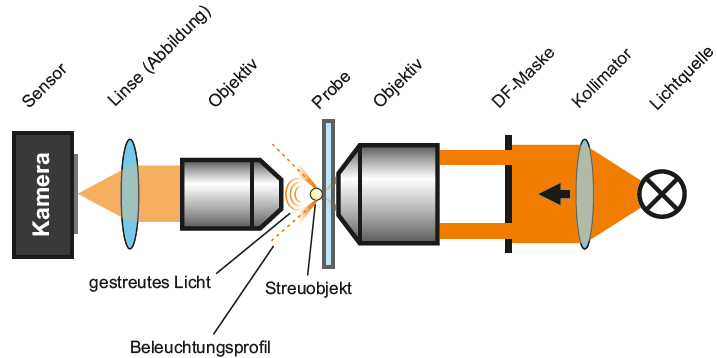
\includegraphics[width=0.8\textwidth]{Dunkel.png}
    \caption{\label{fig:aufbau}Sketch of the beam path of dark field microscope in transmission. 
    The components are labelled, and their functions are described in the main text.}
\end{figure}\FloatBarrier
The DF mask should be brought as close as possible to the first objective to minimize the divergence 
of the transmitted light. This ensures that the analytical specimen does not receive direct light 
from the source, and additionally facilitates the transition between dark field and 
absorption spectroscopy (by removing the mask) since no new adjustment is required. \\

